\documentclass[tikz,border=12pt]{standalone}
\usepackage[T1]{fontenc}
\usepackage{mathpazo}
\usepackage{amsmath,amssymb}
\usetikzlibrary{arrows.meta, calc, decorations.markings}

\definecolor{stblue}{HTML}{7B97AD}
\definecolor{rwgold}{HTML}{B8995E}
\definecolor{sage}{HTML}{7A9A7E}
\definecolor{dkbrown}{HTML}{3D3530}
\definecolor{wmgray}{HTML}{7B7067}
\definecolor{cream}{HTML}{F9F6F0}
\definecolor{border}{HTML}{D4C9B8}
\definecolor{terracotta}{HTML}{C47A6A}
\definecolor{lavender}{HTML}{907EA0}

\begin{document}
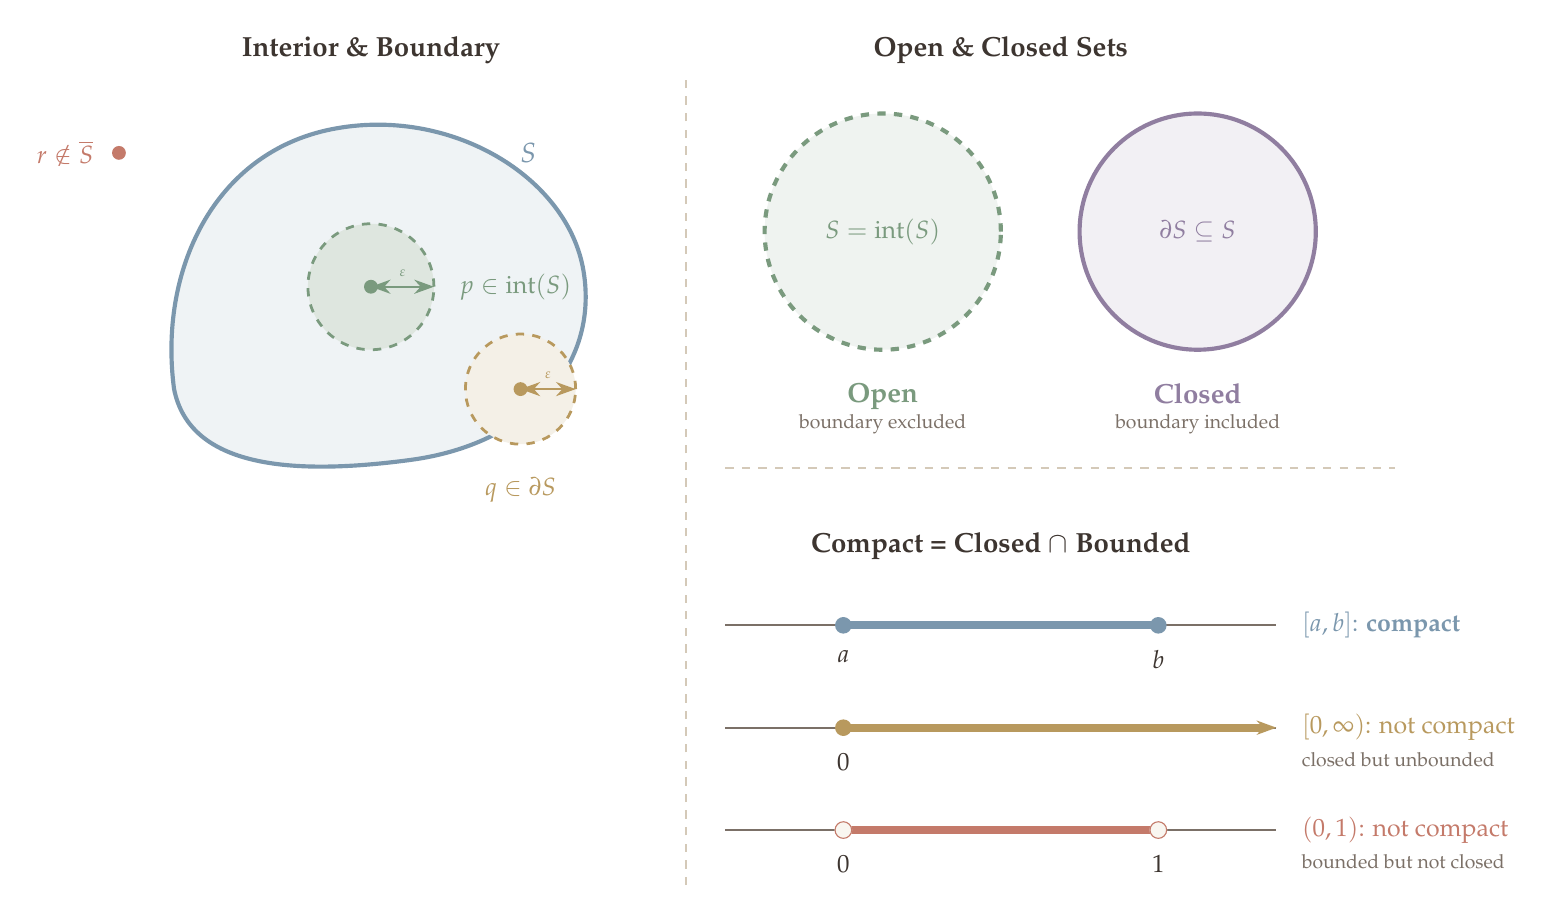
\begin{tikzpicture}[>={Stealth[length=2.5mm, width=1.8mm]}]

% =====================================================
% Panel 1: Interior, Boundary, and Exterior
% =====================================================
\node[font=\normalsize\bfseries, text=dkbrown] at (3.5,5.8) {Interior \& Boundary};

% Set S (smooth blob using Bezier)
\fill[stblue!12]
  (1,1.5) .. controls (0.8,3) and (1.5,4.5) .. (3,4.8)
  .. controls (4.5,5.1) and (6,4.2) .. (6.2,3)
  .. controls (6.4,1.8) and (5.5,0.8) .. (4,0.6)
  .. controls (2.5,0.4) and (1.2,0.5) .. cycle;
\draw[stblue, line width=1.5pt]
  (1,1.5) .. controls (0.8,3) and (1.5,4.5) .. (3,4.8)
  .. controls (4.5,5.1) and (6,4.2) .. (6.2,3)
  .. controls (6.4,1.8) and (5.5,0.8) .. (4,0.6)
  .. controls (2.5,0.4) and (1.2,0.5) .. cycle;

% Label the set
\node[stblue, font=\normalsize] at (5.5,4.5) {$S$};

% Interior point p with epsilon-ball
\fill[sage!25] (3.5,2.8) circle (0.8);
\draw[sage, line width=1pt, dashed] (3.5,2.8) circle (0.8);
\fill[sage] (3.5,2.8) circle (2.5pt);
\node[sage, font=\small, anchor=west] at (4.5,2.8) {$p \in \mathrm{int}(S)$};
\draw[sage, <->, line width=0.6pt] (3.5,2.8) -- node[above, font=\tiny] {$\varepsilon$} (4.3,2.8);

% Boundary point q with epsilon-ball
\fill[rwgold!15] (5.4,1.5) circle (0.7);
\draw[rwgold, line width=1pt, dashed] (5.4,1.5) circle (0.7);
\fill[rwgold] (5.4,1.5) circle (2.5pt);
\node[rwgold, font=\small, anchor=north] at (5.4,0.5) {$q \in \partial S$};
\draw[rwgold, <->, line width=0.6pt] (5.4,1.5) -- node[above, font=\tiny] {$\varepsilon$} (6.1,1.5);

% Exterior point r
\fill[terracotta] (0.3,4.5) circle (2.5pt);
\node[terracotta, font=\small, anchor=east] at (0.1,4.5) {$r \notin \overline{S}$};

% =====================================================
% Panel 2: Open vs. Closed Sets
% =====================================================
\node[font=\normalsize\bfseries, text=dkbrown] at (11.5,5.8) {Open \& Closed Sets};

% Open set (dashed boundary)
\fill[sage!12] (10,3.5) circle (1.5);
\draw[sage, line width=1.5pt, dashed] (10,3.5) circle (1.5);
\node[sage, font=\small] at (10,3.5) {$S = \mathrm{int}(S)$};
\node[sage, font=\normalsize\bfseries, anchor=north] at (10,1.7) {Open};
\node[wmgray, font=\scriptsize, anchor=north] at (10,1.3) {boundary excluded};

% Closed set (solid boundary)
\fill[lavender!12] (14,3.5) circle (1.5);
\draw[lavender, line width=1.5pt] (14,3.5) circle (1.5);
\node[lavender, font=\small] at (14,3.5) {$\partial S \subseteq S$};
\node[lavender, font=\normalsize\bfseries, anchor=north] at (14,1.7) {Closed};
\node[wmgray, font=\scriptsize, anchor=north] at (14,1.3) {boundary included};

% =====================================================
% Panel 3: Compact = Closed + Bounded (number line examples)
% =====================================================
\node[font=\normalsize\bfseries, text=dkbrown] at (11.5,-0.5) {Compact = Closed $\cap$ Bounded};

% Example 1: [a,b] — compact
\draw[wmgray, line width=0.6pt] (8,-1.5) -- (15,-1.5);
\draw[stblue, line width=3pt] (9.5,-1.5) -- (13.5,-1.5);
\fill[stblue] (9.5,-1.5) circle (3pt);
\fill[stblue] (13.5,-1.5) circle (3pt);
\node[dkbrown, font=\small, anchor=north] at (9.5,-1.7) {$a$};
\node[dkbrown, font=\small, anchor=north] at (13.5,-1.7) {$b$};
\node[stblue, font=\small, anchor=west] at (15.2,-1.5) {$[a,b]$: \textbf{compact}};

% Example 2: [0,∞) — closed, not bounded
\draw[wmgray, line width=0.6pt] (8,-2.8) -- (15,-2.8);
\draw[rwgold, line width=3pt] (9.5,-2.8) -- (14.5,-2.8);
\draw[rwgold, ->, line width=3pt] (14.5,-2.8) -- (15,-2.8);
\fill[rwgold] (9.5,-2.8) circle (3pt);
\node[dkbrown, font=\small, anchor=north] at (9.5,-3) {$0$};
\node[rwgold, font=\small, anchor=west] at (15.2,-2.8) {$[0,\infty)$: not compact};
\node[wmgray, font=\scriptsize, anchor=west] at (15.2,-3.2) {closed but unbounded};

% Example 3: (0,1) — bounded, not closed
\draw[wmgray, line width=0.6pt] (8,-4.1) -- (15,-4.1);
\draw[terracotta, line width=3pt] (9.5,-4.1) -- (13.5,-4.1);
\draw[cream, fill=cream] (9.5,-4.1) circle (3pt);
\draw[terracotta] (9.5,-4.1) circle (3pt);
\draw[cream, fill=cream] (13.5,-4.1) circle (3pt);
\draw[terracotta] (13.5,-4.1) circle (3pt);
\node[dkbrown, font=\small, anchor=north] at (9.5,-4.3) {$0$};
\node[dkbrown, font=\small, anchor=north] at (13.5,-4.3) {$1$};
\node[terracotta, font=\small, anchor=west] at (15.2,-4.1) {$(0,1)$: not compact};
\node[wmgray, font=\scriptsize, anchor=west] at (15.2,-4.5) {bounded but not closed};

% Dividing line between top panels
\draw[border, line width=0.5pt, dashed] (8.0,0.5) -- (16.5,0.5);

% Dividing line between left panel and right panels
\draw[border, line width=0.5pt, dashed] (7.5,-4.8) -- (7.5,5.5);

\end{tikzpicture}
\end{document}
